\documentclass{jhwhw}
	\usepackage{enumitem}
	\usepackage{soul}
	\usepackage{graphicx}
	
	\title{CSCI 5271 Exercise Set 1}
    \author{Alex Biedny}
    \date{\today}
    \chead{CSCI 5271 Exercise Set 1}
    \lhead{Alex Biedny}
    
\begin{document}

\maketitle

\problem{Threat Models and Risk Assesment}
Several security goals can be identified:
\begin{itemize}
\item Confidentiality: The contents of the database should only be accessible to the instructor.
\item Availability: The instructor should be able to read and write data in the database.
\item Integrity: Only the instructor should be able to write to the database.
\end{itemize}
Given that this is a small database used for a single college course, the most likely attacker would be a student, likely one enrolled in the course, as they are most likely to have a motivation to attack. From this potential attacker, a reasonable attack would not be very sophisticated, as the attackers would not have the resources to launch any large scale attack. Reasonable attacks to expect would be things like small-scale attempts to brute force a password and attempts to guess the password. Any threats coming from a more sophisticated actor (like a government) shouldn't be considered, as any attempt to mitigate them would be more costly than is worth. As the database is exclusively accessed by the instructor and there is no public user input used to read/write database information, attacks like SQL injection need not be considered also.
\\
If the database is on a laptop with no internet or network connection and no floppy drive (I take this to mean it has no way to transfer external data onto the laptop), the only threats to the database security would be from users physically using the laptop. From this, a few security mechanisms will help acheive the security goals:
\begin{itemize}
\item In order to keep the database confidential and maintain integrity of data, authentication can be required before reading from or writing to it. This will have no monetary cost, as most modern database engines are free and come with systems that can require authentication to access the database. This will cost some time to initially set up, and will affect the goal of Availability by slowing down the instructors ability to access to database by requiring authentication.
\item To further the goals of confidentiality and data integrity, the security features of the operating system that the laptop runs can be used. Modern operating systems all offer some sort of user account system that is able to make certain files accessible to only authorized users. By utilizing this, access to the database files themselves can be restricted to only authorized users of the OS. This mechanism will also have no monetary cost, and will only cost time to set up and time to enter a password before accessing the database.
\item As the laptop has no ability to network, if it is physically inaccessible to attackers, there will be no way to attack the database. The instructor could use a laptop lock to ensure that it cannot physically cannot leave a certain area, in which case any potential attack would require the attackers to be where the laptop and lock are. This will have some monetary cost, but a very low one on the order of \$20-\$50.
\end{itemize}

\problem{Finding vulnerabilities}
\begin{enumerate}
\item The vulnerability in this comes from the line executing the \verb last  command. In order to exploit this, your input to the program (which is recieved through STDIN) should be of the form \verb any_string=;command_to_run  where \verb any_string  is any string (is never used by the script after being assigned) and where \verb command_to_run  is the abitrary command to be executed.
\\
After the input from STDIN is read, the script splits the input string based on the character \verb =  and then uses the second substring returned directly in the command \verb^$result = ‘last -1000 | grep $username_to_look_for‘;^ in place of \\\verb^$username_to_look_for.^ By including a semicolon in the input, when the command is evaluated, the \verb^grep^ command will run with no input, as the semicolon indicates the end of the command. Then, anything included after the semicolon will be evaluated as a command and ran with the programs privledges. 
\\
To avoid this problem, the script should first sanitize the input to make sure no special characters that could cause unexpected execution of commands are in the input string. As this is looking for a username, it would likely be wise to restrict the set of characters users are allowed to enter.

\item This function makes two checks to make sure that \verb pathname  is not a path to the file \verb /what/ever/ , the first before it reads in the file at \verb pathname  and the second before the buffer containing the contents of the file - 1 byte from the end is written back to it.
\\
To exploit a race condition, you should first pass in any path name that is not \verb /what/ever/ . After the first check to make sure that \verb pathname  is not \verb /what/ever/  is passed, as \verb pathname  is a pointer you are able to change the data at the memory it points to. This should be changed to \verb /what/ever/  before the line \verb^rfd = open(pathname, O_RDONLY);^ is executed, and then changed back after the line executes. Because of this, the \verb open  call will return a file descriptor to \verb /what/ever/ and the subsequent line will use that file descriptor to read in all but the last byte of its data, even after \verb pathname  has been changed back.
\\
Next, \verb pathname  should be changed a final time to \verb /what/ever/  right after the line \verb^stat(pathname, &f);^ executes. This will allow the next check that the file to be altered is not \verb /what/ever/  to pass, and by the time \verb^wfd = open(pathname, O_WRONLY | O_TRUNC);^ executes, \verb pathname  will be \verb /what/ever/  , meaning that it will be overwritten with a buffer containing itself, sans the last byte.
\end{enumerate}

\problem{Overflowing buffers}
\begin{enumerate}
\item With the stack growing in the opposite direction, you'd no longer be able to overwrite the return address of the function currently executing. However, as the stack now grows up, any time a function is called the new function frame will be at a higher set of memory addresses than the calling function frame. This means you can exploit a buffer overflow to overwrite parts of the next function frame - including the return address. 
\\
When \verb^strcpy()^ is called, it is pushed to the top of the stack, at a higher set of addresses than the calling function. Its return address is copied to the usual place in its function frame, and the stack would look like what is shown below:
\begin{center}
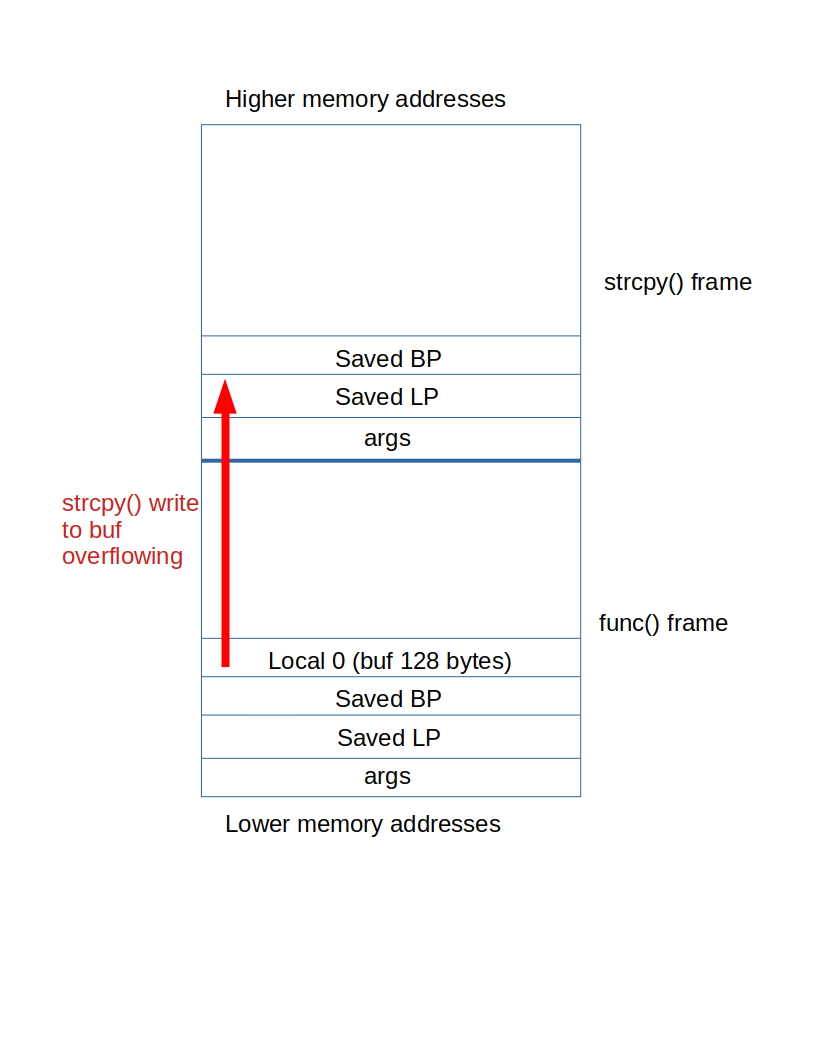
\includegraphics[scale=0.25]{HW1_1.png}
\end{center}
To take over control flow, the input \verb^str^ should be long enough to fill \verb^buf^ with a \verb^nop^ slide, then whatever shellcode you would like to execute, and then junk data until the write reaches the return address of \verb^strcpy()^'s frame, in which it should replace the real return address with the address of the buffer that is now filled with shellcode.
\\ The control flow of the program would start normally, until \verb^strcpy()^ is called. A new function frame would be pushed to the top of the stack, arguments and return addresses copied over, and then execution would start in the \verb^strcpy()^ function. This would execute as normal, writing the input to \verb^buf^ until it overflows, all the way until it overflows into the next stack frame and overwrites that return address with whatever is intended. The \verb^strcpy()^ function would then complete and return, but as the return address has been overwritten, the computer will execute whatever data is at that address, and control flow has been hijacked.

\item Because this system uses canaries, it is not possible to use an overflowing write to overwrite things like return addresses. However, it is still possible to overwrite local variables, and this can be exploited to allow more than 100 connections in the given function.
\\
To exploit this, the input \verb^user^ should contain first 128 bytes of junk data in order to fill up \verb^buf^, and then should contain the 32-bit (assuming that the size of \verb^int^ in this system is 32-bit) two's complement representation of a number less than 100. This number will also have to be represented in the same endianness of the system. This will overwrite the variable \verb^tmp^, which is later used in an if statement to check if there are less than 100 connections. Thus even if \verb^total_connections^ is already at or above 100, the function will allow another connection.
\end{enumerate}

\problem{Nondefensive programming}
\begin{enumerate}
\item There are several bugs in this code that could be exploited by an attacker. First, the variable \verb^len^ is declared as a signed integer, despite being intended to store length. It is then assigned the result of the \verb^strlen(a)^ function. As \verb^a^ is an input to the function, it could be a long enough string to cause \verb^len^ to overflow to a negative number. In addition, the value of \verb^len^ is then used as an argument to a \verb^malloc()^ call. If \verb^len^ is negative or too large of a number when this happens, the \verb^malloc()^ will fail. On top of that, the return value from \verb^malloc()^ is never checked, so if it fails and returns a null pointer the function will not know, and this will eventually lead to a null pointer dereference.
\\
Even if the \verb^malloc()^ call returns as expected, there are other bugs. The length of \verb^b^ is never checked, and it could be anything - like a null pointer. It is then repeatedly dereferenced in the for loop. In addition to this, the for loop uses \verb^i <= len^ for its comparison. Because of this, even if there are no problems with \verb^malloc()^ and \verb^b^, on the loops last iteration when \verb^i^ = \verb^len^, the loop will try to assign beyond even the expected bounds of the \verb^result^ array, and \verb^a[i]^ and \verb^b[i]^ will have vales read from beyond their bounds.
\\ A better implementation of this could be something like this:
\begin{verbatim}
char *zip(const char *a, const char *b) {
  uint32_t lenA = strlen(a);
  uint32_t lenB = strlen(b);
  if (lenA != lenB) return -1; //error
  char *result = malloc(lenA + lenB + 1);
  if (!result) return -1; //error
  for (uint32_t i = 0; i < lenA + lenB; i += 2) {
    result[i] = a[i];
    result[i+1] = b[i];
  }
  result[lenA + lenB] = '\0';
  return result;
}
\end{verbatim}
\item First, as the do-while loop checks the loop condition at the end, if one or both of \verb^input1^ or \verb^input2^ are null, the body of the loop will dereference them before the loop breaks.
\\
Next, the \verb^strcmp()^ function is used to compare data in the links, the \verb^strncmp()^ function should be used instead, as the input strings may not be properly null-terminated.
\\
When the \verb^strcmp()^ function is used, it is used to compare the strings in the list nodes to keep them sorted. As characters will be compared here using ASCII codes, the sorting may not be alphabetical, or what was intended.
\\
At the start of the function, there is no null check for \verb^input1^ and \verb^input2^ before the are dereferenced.
\\
After the loop, there is no check to see if \verb^input2^ is not null like there is with \verb^input1^.
\end{enumerate}

\end{document}